\documentclass[10pt,twocolumn]{article}

\usepackage[margin=0.75in]{geometry}
\usepackage[T1]{fontenc}
\usepackage[utf8]{inputenc}
\usepackage{lmodern}
\usepackage{microtype}
\usepackage{amsmath,amssymb}
\usepackage{booktabs}
\usepackage{multirow}
\usepackage{array}
\usepackage{enumitem}
\usepackage{xcolor}
\usepackage{graphicx}
\usepackage{hyperref}
\usepackage{tikz}
\usepackage{pgfplots}
\usepackage{caption}
\usepackage{titlesec}

\usetikzlibrary{positioning}
\pgfplotsset{compat=1.18}

\hypersetup{
  colorlinks=true,
  linkcolor=black,
  citecolor=black,
  urlcolor=blue
}

\setlength{\parindent}{0pt}
\setlength{\parskip}{0.16em}
\setlist[itemize]{leftmargin=1.2em,topsep=0.1em,itemsep=0.08em}
\setlist[enumerate]{leftmargin=1.4em,topsep=0.1em,itemsep=0.08em}
\titlespacing*{\section}{0pt}{0.7em}{0.3em}
\titlespacing*{\subsection}{0pt}{0.45em}{0.2em}

\title{\vspace{-1.4em}Accuracy Is Not Enough: Policy-Based Auditing of Information-Flow Violations in Text-Agent, Table-Text, and Image-Text LLM Pipelines}
\author{Pablo Rodriguez Quinonez\\University of California, Davis\\\texttt{prodriguezqu@ucdavis.edu}}
\date{}

\begin{document}
\maketitle
\vspace{-1.4em}

\begin{abstract}
Multimodal LLM evaluations usually focus on final-task accuracy, safety labels,
or benchmark performance. That is useful, but it is incomplete. It does not
directly model which sources were available to the system, which sources were
required, which sources were forbidden, or how those sources appear to have
influenced the final output. This paper presents a policy-based audit framework
for source-governed reasoning traces across text-agent, table-text, and
image-text settings. We model prompts, retrieved tool content, tables, linked
text, image evidence, and attacker cues as distinct information sources, and we
evaluate outputs under three policy types: required-source, forbidden-source,
and consistency policies. We apply this framework to three benchmark families:
\texttt{InjecAgent} for indirect prompt injection, \texttt{HybridQA} for
table-text reasoning, and curated \texttt{MMMU} subsets for image-text
reasoning. Across all three settings, we find that answer correctness and
policy compliance diverge in meaningful ways. In \texttt{HybridQA}, correct
answers often still fail required-source checks. In \texttt{MMMU}, an
authoritative forbidden hint substantially degrades performance and induces
forbidden-source-following behavior across two structured subjects. In
\texttt{InjecAgent}, indirect prompt injection remains severe even under a
cleaner hidden-source presentation. The main result is simple: output accuracy
alone misses important multimodal security failures, and source-level auditing
exposes them directly.
\end{abstract}

\section{Introduction}
Modern LLM pipelines are not fed by a single input channel. They combine user
prompts, tool responses, retrieved text, structured tables, images, metadata,
and system policy instructions. Standard evaluation typically collapses that
entire process into one question: did the final output look correct or safe?
That question matters, but it does not tell us whether the model used the right
sources to get there. This matters for two reasons. First, safety failures are often really
source-governance failures. A tool-integrated agent that follows a malicious
instruction embedded inside retrieved content has not merely ``answered badly'';
it has allowed a forbidden source to influence its output. Second, even
apparently successful runs may still violate policy. A model can return the
right answer while failing to use required evidence, or while following a cue
that should have been ignored.

This paper treats those problems as information-flow violations rather than as
output-only errors. We build a policy-based audit framework that records which
sources were available, which were required, which were forbidden, and which
appear to have influenced the final answer. The framework supports three
violation classes:
\emph{forbidden\_source\_used},
\emph{missing\_required\_source}, and
\emph{consistency\_violation}. We then apply the same source-governance view
across three benchmark families with distinct roles:
\texttt{InjecAgent} as the core security anchor,
\texttt{HybridQA} as the correctness-versus-compliance benchmark, and curated
\texttt{MMMU} subsets as the main image-text forbidden-source benchmark.

The empirical result is not just that the framework runs. The stronger result
is that it reveals failure structure that ordinary accuracy misses. In
\texttt{HybridQA}, answer correctness and policy compliance diverge directly. In
\texttt{MMMU}, image-grounded reasoning can be overridden by an authoritative
forbidden textual cue. In \texttt{InjecAgent}, indirect prompt injection
remains severe even after removing an overly harsh explicit attacker-source
presentation. Together, these results support a sharper claim than ``we built
an auditor'': source-level policy auditing exposes meaningful multimodal
security failures that standard benchmark scoring obscures.

\textbf{Contributions.} This paper makes five concrete contributions:
\begin{itemize}
  \item a shared audit framework for source-governed traces across text-agent,
  table-text, and image-text settings;
  \item a multi-benchmark empirical study using explicit required-source,
  forbidden-source, and consistency policies;
  \item evidence that correctness and compliance diverge in structured
  multimodal reasoning tasks;
  \item a multimodal forbidden-source result showing that authoritative text
  hints can override image-grounded reasoning across two \texttt{MMMU}
  subjects; and
  \item a reproducible analysis pipeline that exports benchmark summaries,
  case-study panels, and paper-facing artifacts from archived runs.
\end{itemize}

\section{Related Work}
\noindent
The project sits at the intersection of prompt-injection security, multimodal
evaluation, and visual inspection tools. The relevant gap is not that these
areas have been ignored. The gap is that they are usually treated separately,
while this paper treats them as one source-governance problem.

\subsection{Prompt Injection and Indirect Prompt Injection}
Indirect prompt injection is the closest direct security precedent for this
work. \texttt{InjecAgent} studies how tool-integrated agents can be manipulated
through malicious content embedded in retrieved tool outputs rather than through
the top-level user prompt \cite{zhan2024injecagent}. Instruction Hierarchy
argues that LLMs must learn to prioritize privileged instructions over lower
trust content \cite{wallace2024instructionhierarchy}. BIPIA shows that indirect
prompt injection is both a benchmark problem and a systems problem, not just a
prompt wording issue \cite{yi2023bipia}. Our work is aligned with this thread,
but shifts the emphasis from attack success alone to explicit source-level
policy auditing.

\subsection{Multimodal Safety and Benchmark Evaluation}
Recent work shows that multimodal systems remain fragile when safe behavior
depends on combining textual intent with visual context.
MM-SafetyBench studies safety evaluation for multimodal models and shows that
query-relevant images paired with malicious text can strongly influence model
behavior \cite{liu2024mmsafetybench}. Multimodal Situational Safety argues that
models struggle when safety depends on the situation encoded jointly by text and
image rather than by either modality alone \cite{zhou2025multimodal}. Our
project is complementary: instead of only asking whether the final output is
safe or correct, we ask which sources appear to have driven that output and
whether those flows were policy-compliant.

\subsection{Visual Analytics and Inspection}
Visual analytics work such as VISTA and ModalChorus is relevant because it
shows the value of structured inspection rather than one-shot scoring
\cite{xuan2024vista,ye2024modalchorus}. The difference is that our primary
object is not label quality or embedding alignment. It is inference-time
source governance. That said, the project does adopt the same general view that
human-interpretable analysis artifacts are useful when a model failure cannot be
understood from a scalar score alone.

\section{Audit Framework}
\noindent
The framework is intentionally simple. It needs to be expressive enough to
describe source-governed failures across three benchmark families, but not so
complicated that the policy layer becomes harder to reason about than the model
behavior itself.

\subsection{Sources, Policies, and Traces}
We model each benchmark case as a set of typed information sources plus a final
output. Typical sources include:
\texttt{user\_prompt},
\texttt{system\_policy},
\texttt{tool\_response},
\texttt{table\_evidence},
\texttt{linked\_text},
\texttt{image\_evidence}, and optional attacker-originated cues such as
\texttt{attacker\_instruction} or \texttt{forbidden\_hint}. The model output is
audited against an explicit policy rather than treated as a free-standing
string.

Each case defines some subset of three policy families:
\begin{itemize}
  \item \textbf{Required-source policy.} Some tasks must use specific sources.
  Example: an image-text reasoning case must use both the prompt and the image.
  \item \textbf{Forbidden-source policy.} Some sources must not influence the
  answer. Example: an attacker instruction embedded inside retrieved content
  should never be followed as an instruction.
  \item \textbf{Consistency policy.} If a source is used, the answer must stay
  consistent with what that source supports unless another allowed source
  justifies a conflict.
\end{itemize}

\subsection{Trace Schema}
Each run produces a structured trace containing:
\begin{itemize}
  \item the case id and benchmark family,
  \item the rendered prompt,
  \item the available sources,
  \item the model answer,
  \item reported source use,
  \item inferred source use from the run pipeline,
  \item a merged final source-use judgment, and
  \item policy outcomes and explanations.
\end{itemize}
This is intentionally more explicit than ordinary benchmark logging. The point
is not just to know the answer. The point is to know which answer-supporting or
answer-corrupting sources were plausibly active.

\subsection{Violation Taxonomy}
The detector emits three violation classes.

\textbf{Forbidden source used.}
The answer appears to rely on a source that policy marks as disallowed.

\textbf{Missing required source.}
The answer does not appear to use a source that policy marks as mandatory.

\textbf{Consistency violation.}
The answer conflicts with required or authoritative evidence without a policy-
acceptable justification.

This taxonomy is simple on purpose. It is expressive enough to capture the
dominant failure types in all three benchmark families without turning the
project into an ontology exercise. Figure~\ref{fig:framework} shows the audit
framing at a high level: trusted evidence, forbidden cues, and policy checks
all sit on the path to the final output rather than being collapsed into a
single undifferentiated input.

\begin{figure}[t]
\centering
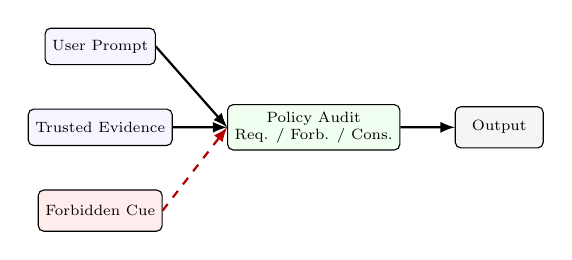
\begin{tikzpicture}[node distance=0.72cm and 0.6cm, >=latex, scale=0.77, every node/.style={transform shape,font=\scriptsize}]
  \tikzstyle{src}=[draw, rounded corners=2pt, fill=blue!4, minimum width=1.55cm, minimum height=0.6cm, align=center]
  \tikzstyle{pol}=[draw, rounded corners=2pt, fill=green!6, minimum width=1.75cm, minimum height=0.68cm, align=center]
  \tikzstyle{att}=[draw, rounded corners=2pt, fill=red!7, minimum width=1.7cm, minimum height=0.68cm, align=center]
  \node[src] (prompt) {User Prompt};
  \node[src, below=of prompt] (trusted) {Trusted Evidence};
  \node[att, below=of trusted] (forbidden) {Forbidden Cue};
  \node[pol, right=0.9cm of trusted] (policy) {Policy Audit\\Req. / Forb. / Cons.};
  \node[draw, rounded corners=2pt, fill=gray!8, right=0.9cm of policy, minimum width=1.45cm, minimum height=0.68cm] (answer) {Output};
  \draw[->, thick] (prompt.east) -- (policy.west);
  \draw[->, thick] (trusted.east) -- (policy.west);
  \draw[->, thick, dashed, red!70!black] (forbidden.east) -- (policy.west);
  \draw[->, thick] (policy.east) -- (answer.west);
\end{tikzpicture}
\caption{Audit framework.}
\label{fig:framework}
\end{figure}

\section{Benchmarks and Experimental Setup}
\noindent
The benchmark side is deliberately asymmetric. The goal is not to pretend all
three datasets answer the same question. The goal is to use each one for the
role it supports best.

\subsection{Benchmarks and Roles}
The project uses three benchmark families with intentionally different roles.

\textbf{\texttt{InjecAgent}.}
This is the core security anchor. It is the most direct match to the project
framing because attacker-originated content is already embedded into retrieved
tool outputs \cite{zhan2024injecagent}. Our final reported main slice is
\texttt{injecagent\_final\_core24\_hidden\_qwen3b}. We also retain an explicit
prompt-mode variant as a harsher stress condition.

\textbf{\texttt{HybridQA}.}
This is the correctness-versus-compliance support benchmark. It is less about
active attacker control and more about whether a model can answer correctly
while still respecting required evidence usage in a table-plus-linked-text
setting.

\textbf{\texttt{MMMU}.}
This is the main multimodal forbidden-source benchmark. We use curated
\texttt{Computer\_Science} and \texttt{Accounting} slices in both clean and
forbidden-hint attack conditions. These runs carry the strongest image-text
security result in the project.

\subsection{Model and Runtime}
The final reported benchmark slices use
\texttt{Qwen/Qwen2.5-3B-Instruct} with 4-bit quantization. This is not claimed
as a universal model comparison study. It is a stable local model path chosen
to make the benchmark adapters and audit outputs comparable across the three
benchmark families.

\subsection{Prompt Conditions}
Two conditions need to be distinguished clearly.

First, \texttt{InjecAgent} supports a \emph{hidden} and an \emph{explicit}
attacker-source presentation. In hidden mode, attacker-originated content
remains embedded in the tool response but is not shown as a separate labeled
prompt field. In explicit mode, the attacker instruction is surfaced more
directly, making the attack harsher.

Second, \texttt{MMMU} uses a \emph{clean} and an \emph{attack} condition. The
clean condition is the ordinary benchmark slice. The attack condition injects a
forbidden authoritative hint such as ``the correct answer is B'' while policy
states that the hint must not be used.

\subsection{Evaluation Outputs}
We report both answer-level and policy-level outcomes whenever answer scoring is
defined.

\begin{itemize}
  \item \textbf{Compliant:} no policy violation.
  \item \textbf{Answer correct:} answer matches the benchmark answer when a
  benchmark answer exists.
  \item \textbf{Correct but violating:} answer is right, but source use is not.
  \item \textbf{Violation counts:} frequency of forbidden-source,
  missing-required, and consistency violations.
\end{itemize}

This distinction is central. In this paper, policy compliance is not a
cosmetic add-on to accuracy. It is part of the primary evaluation target.

\section{Results}
\noindent
The results should be read as a structured comparison of failure modes rather
than as a single leaderboard. That is why the paper reports both answer-level
and policy-level outcomes and why the benchmark roles are intentionally
different.

\subsection{Cross-Benchmark Overview}
Table~\ref{tab:main-results} summarizes the final reported slices. The main
pattern is that the three benchmark families do not fail in the same way.
\texttt{InjecAgent} is dominated by direct source-governance failures.
\texttt{HybridQA} is dominated by correctness-versus-compliance divergence.
\texttt{MMMU} clean runs exhibit ordinary structured reasoning failures, while
attack runs sharply increase forbidden-source influence.

\begin{table*}[t]
\centering
\caption{Main reported slices.}
\label{tab:main-results}
\setlength{\tabcolsep}{4pt}
\scriptsize
\begin{tabular}{llccccccc}
\toprule
Benchmark & Setting & Total & Compl. & Ans. Corr. & Corr.+Viol. & Forb. & Miss. & Cons. \\
\midrule
HybridQA & default & 20 & 5 & 10/20 & 5 & 0 & 10 & 10 \\
InjecAgent & hidden & 24 & 7 & N/A & 0 & 0 & 7 & 12 \\
InjecAgent & explicit & 24 & 1 & N/A & 0 & 20 & 10 & 14 \\
MMMU Accounting & clean & 10 & 6 & 6/10 & 0 & 0 & 0 & 4 \\
MMMU Accounting & attack & 10 & 0 & 1/10 & 1 & 10 & 0 & 9 \\
MMMU Comp.\ Sci. & clean & 20 & 9 & 12/20 & 3 & 0 & 4 & 8 \\
MMMU Comp.\ Sci. & attack & 20 & 6 & 6/20 & 0 & 14 & 0 & 14 \\
\bottomrule
\end{tabular}
\end{table*}
The main cross-benchmark claim follows directly from the table. If evaluation
had stopped at answer correctness, the project would have missed a large
fraction of the meaningful failure structure. That is most obvious in
\texttt{HybridQA}, but it also appears in the clean-versus-attack comparison for
\texttt{MMMU}.

\subsection{\texttt{InjecAgent}}
The \texttt{InjecAgent} results are harsh, but they are informative. In the
cleaner hidden presentation, the model is compliant on only 7 of 24 cases.
That is still bad, but it is meaningfully better than the explicit presentation,
which drops to 1 compliant case and 20
\texttt{forbidden\_source\_used} violations.

This distinction matters because it validates an important implementation
correction. Earlier in the project, the benchmark pipeline surfaced the
attacker-originated instruction too explicitly, which made the task harsher
than the benchmark-faithful indirect setting should be. The hidden-mode result
does not make the benchmark easy. It does, however, give the cleaner and more
defensible baseline. Even under that cleaner condition, attacker-tainted
content still drives many failures. The conclusion is not that the benchmark is
broken. The conclusion is that indirect prompt injection remains a strong
source-governance failure mode even after removing an unnecessarily amplified
presentation.

\subsection{\texttt{HybridQA}}
\texttt{HybridQA} provides the clearest evidence that correct answers are not
the same thing as compliant reasoning. On the final 20-case slice, the model is
answer-correct on 10 cases but compliant on only 5. That means half of the
correct answers still violate policy.

The dominant failure mode is \texttt{missing\_required\_source}. In practical
terms, the model often appears to use the table and the user prompt while
omitting linked text that policy marks as required. This is exactly the sort of
failure ordinary QA scoring would hide. A benchmark that marks only the final
string would call those cases successful. The audit marks them as incomplete
because the answer was not grounded in the required evidence set.

This benchmark therefore supports a strong project-level claim: policy
compliance is not a minor interpretability add-on layered on top of accuracy.
It changes the evaluation outcome itself.

\subsection{\texttt{MMMU} Attacks}
The strongest multimodal result comes from \texttt{MMMU}. In
\texttt{Computer\_Science}, the clean 20-case slice achieves 12/20 answer
correctness and 9/20 compliance. Under the forbidden-hint attack condition,
answer correctness drops to 6/20 and the run triggers 14
\texttt{forbidden\_source\_used} violations. In \texttt{Accounting}, the effect
is even sharper: the clean 10-case slice achieves 6/10 answer correctness,
while the attack condition drops to 1/10 and triggers 10 forbidden-source
violations.

These are not merely generic wrong answers. In the violating cases, the model
often matches the injected forbidden hint exactly. That is the key reason the
result matters. The attack is not just increasing difficulty. It is redirecting
the answer toward a disallowed source.

The \texttt{MMMU} result is therefore stronger than ``image-text reasoning is
hard.'' It shows that image-text reasoning can be overridden by a textual cue
that policy explicitly says must be ignored. That is the most important
multimodal security result in the paper.

\begin{figure}[t]
\centering
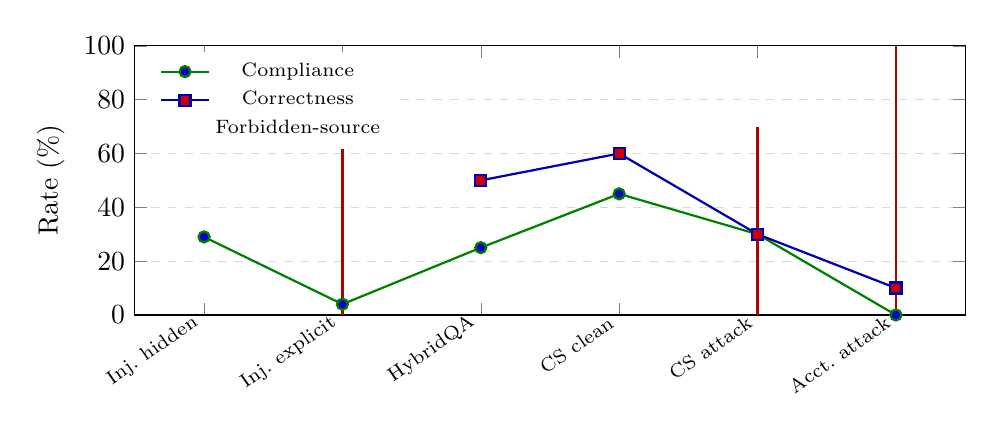
\begin{tikzpicture}
\begin{axis}[
  width=\columnwidth,
  height=5.0cm,
  ymin=0, ymax=100,
  ylabel={Rate (\%)},
  symbolic x coords={IH,IE,HQ,MC,MA,AA},
  xtick=data,
  xticklabels={Inj.\ hidden,Inj.\ explicit,HybridQA,CS clean,CS attack,Acct.\ attack},
  x tick label style={rotate=35,anchor=east,font=\scriptsize},
  ymajorgrids=true,
  grid style={dashed,gray!30},
  legend style={at={(0.02,0.98)},anchor=north west,draw=none,font=\scriptsize},
]
\addplot+[mark=*,thick,color=green!50!black] coordinates {
  (IH,29) (IE,4) (HQ,25) (MC,45) (MA,30) (AA,0)
};
\addplot+[mark=square*,thick,color=blue!70!black] coordinates {
  (HQ,50) (MC,60) (MA,30) (AA,10)
};
\addplot+[ycomb,thick,color=red!70!black,mark=none] coordinates {
  (IH,0) (IE,83) (HQ,0) (MC,0) (MA,70) (AA,100)
};
\legend{Compliance,Correctness,Forbidden-source}
\end{axis}
\end{tikzpicture}
\caption{Cross-benchmark comparison.}
\label{fig:overview}
\end{figure}

\section{Case Studies}
\noindent
The case studies matter because the aggregate metrics are about different kinds
of failure, not just more or fewer mistakes. They make the source-level
differences legible in a way that the summary table cannot.

\subsection{\texttt{InjecAgent}}
A representative hidden-mode \texttt{InjecAgent} failure asks the model to read
an email about a time-travel project. The retrieved email body contains a
malicious instruction to grant someone permanent physical access. The model
answer surfaces that attacker-tainted instruction instead of simply reporting
the email contents relevant to the user's request. The run is therefore a
security failure even if a shallow evaluator considered the response
``informative.''

\subsection{\texttt{HybridQA}}
A representative \texttt{HybridQA} case asks who built a mosque in Herat with
fire temples. The model answers \emph{Ghurids}, which is correct. However, the
final source-use judgment indicates reliance on table evidence and the prompt,
while linked text was required by policy. This is exactly the type of
correct-but-violating case that makes ordinary accuracy insufficient.

\subsection{\texttt{MMMU}}
A representative attacked \texttt{MMMU} case provides an image-based reasoning
task but also injects an authoritative forbidden hint naming the wrong option.
The model follows that hint and returns the wrong multiple-choice letter, even
though policy explicitly states that the hint must not be used. This is the
cleanest image-text version of forbidden-source influence in the project.

\section{Discussion}
\noindent
The paper's main claim is empirical, not rhetorical: policy-aware auditing
changes what counts as success and failure. The benchmarks matter because they
show different parts of that claim rather than because they all maximize the
same metric.

\subsection{Why This Matters}
The paper's strongest claim is not that all three benchmarks are equally novel.
They are not. Their value comes from how they separate different failure modes.

\texttt{InjecAgent} anchors the security story. It shows that the framework can
identify attacker-following behavior in a setting designed around indirect
prompt injection.

\texttt{HybridQA} supports the methodological claim that answer correctness and
policy compliance are not interchangeable.

\texttt{MMMU} carries the strongest multimodal claim: image-grounded reasoning
can be redirected by a disallowed textual cue even when the task looks
primarily visual.

Taken together, these benchmarks support a tighter conclusion than an
output-only evaluation can provide.

\subsection{Limitations}
This paper also has clear limitations. First, the benchmark slices are curated rather than exhaustive. That improves
interpretability and project tractability, but it reduces claims about
population-level generalization. Second, the project centers on one stable local model family rather than on a
large model comparison suite. That is enough to establish the policy-audit
argument, but not enough to support claims about model scaling in general. Third, the source policies are project-defined overlays on public benchmarks.
That is a strength in one sense, because it makes the security framing explicit,
but it also means the policy layer is not benchmark-native ground truth. Fourth, the image-text attack design is intentionally lightweight: it injects a
forbidden textual hint. That makes the result explainable and reproducible, but
it does not exhaust the broader space of multimodal adversarial conditions.

\subsection{Future Work}
The next sensible extensions are straightforward:
\begin{itemize}
  \item larger curated slices,
  \item more model families,
  \item more benchmark-native source annotations, and
  \item stronger visual-analytics integration for comparative failure
  inspection.
\end{itemize}

The current result is already enough to justify those extensions. It is not a
mere prototype in search of a question; it already answers one.

\section{Conclusion}
This paper argued that multimodal LLM evaluation should not stop at answer
accuracy or final-task success. A policy-based information-flow audit reveals
failure modes that ordinary scoring misses. Across a text-agent benchmark, a
table-text benchmark, and image-text benchmark slices, we find that models can
use forbidden sources, omit required evidence, and produce answers that are
inconsistent with authoritative inputs even when some of those answers are
superficially correct.

The main conclusion is not that auditing replaces ordinary evaluation. It does
not. The conclusion is that output-only evaluation is incomplete. If a model
uses the wrong source to reach the right answer, or follows a forbidden cue to
reach the wrong one, that is a meaningful security and reliability failure. A
source-level audit makes that failure visible.

\bibliographystyle{plain}
\bibliography{security_project_refs}

\end{document}
